\section{Results}
\label{sec:DL-results}

\subsection{Hardware and Software setup}
\label{subsec:hardware-software}
To implement the neural networks I used Keras \cite{chollet2015keras}. Keras is an artifitial neural network library written in python programming language. It is designed to be minimalistic, modular and straight forward to use, but yet powerful and generic enough to build serious models. It is built on top of either Theano or Tensorflow. In this work, I used the Theano backend. Theano is a Python library that lets you to define, optimize, and evaluate mathematical expressions, especially ones with multi-dimensional arrays. Using Theano it is possible to attain speeds rivaling hand-crafted C implementations for problems involving large amounts of data. It can also surpass C on a CPU by many orders of magnitude by taking advantage of recent GPUs, using the latest version of CUDA platform. \cite{theano2010} \cite{theano2012}

The work reported in the following sections were performed under the following hardware setup:
\begin{itemize}
\item Microsoft Windows 8.1 Pro (64-bit)
\item Intel Core i7-3770 CPU
\item 32.0GB of RAM
\item GeForce GTX 660 video card
\end{itemize}

\noindent 
and the following software setup:
\begin{itemize}
\item python 3.4.4
\item numpy 1.10.4
\item keras 0.3.2
\item theano 0.8.0dev0
\item CUDA 7.5
\end{itemize}

Only one GPU was utilized when performing the computations in this chapter, however it is worth noting that as of March 2016 Theano added support for multiple GPUs.

\subsection{Data Preparation}
\label{subsec:data-preparation}
The same datasets from the previous chapter were used. First it was necessary to prepare the data to be fed to the Deep Neural Network (DNN).Each dataset was first filtered using the same filter as phy: a forwards-backwards Butterworth filter of order 3 with cutoff frequency set to 500Hz. Each dataset was then normalized dividing by its maximum value, such that every sample has a value between -1 and 1.

Each example was defined to be the array of time windows of 100 samples for each of the 127 channels in the probe. Therefore, the input data has dimension 12700. However, due to constraints on the available hardware, not all windows were used. Each window is shifted by 5 samples from the previous one, i.e., the first example are the 127 time windows with $t \in [ 0 , 99]$ and the second example are the 127 time windows when $t \in [ 5, 104]$. Furthermore, only samples in $t \in [1000000,2000000]$ were utilized. This yields, at this stage, 199980 examples per dataset

The windows whose central sample was closest to each Juxta Times were labeled as "1" (positive examples). This means that the central sample of these windows will be at most two samples  away from the true Juxta Time. Otherwise they were labeled as "0" (negative examples). The label "1" should be interpreted as "contains a spike from the juxta cell" and "0" as "doesn't contain a juxta spike". It is possible that a spike from the juxta cell be partially contained in the window of another spike from the juxta cell. However this situation is highly unlikely since for that to happen it would mean that the two spike were separated by less that 50 samples, corresponding to 1.67 ms which is less than the refractory period of cells under consideration.

This input data was split in two set: the training set (TS), with which the DNN will train, and the validation set (VS), where the resulting trained DNN is tested. The TS held 70\% of the input data (139986 examples) and VS held the remaining 30\% (59994 examples)

In table \ref{table:summary-beforeUS} are the results of this splitting.
\begin{table}[htbp]
\begin{center}
\begin{tabular}{r|cc|cc|cc}
\multicolumn{1}{l|}{} & \multicolumn{ 2}{c|}{Input Data} & \multicolumn{ 2}{c|}{Training Set} & \multicolumn{ 2}{c}{Validation Set} \\ \hline
cell ID & No. of "1"  & Fraction & No. of "1"  & Fraction & No. of "1" & Fraction \\ \hline
8213 & 292 & 0.15\% & 202 & 0.14\% & 90 & 0.15\% \\ 
936 & 127 & 0.06\% & 83 & 0.06\% & 44 & 0.07\% \\ 
939 & 298 & 0.15\% & 207 & 0.15\% & 91 & 0.15\% \\ 
945 & 14 & 0.01\% & 9 & 0.01\% & 5 & 0.01\% \\ 
997 & 38 & 0.02\% & 29 & 0.02\% & 9 & 0.02\% \\ 
\end{tabular}
\end{center}
\caption{In this table are presented, for each recording, the number of examples labeled as "1" and its fraction in the Input Data, and separated in the Training Set and Validation Set. The total number of examples in the Input Data, Training Set and Validation Set are 199980, 139986 and 59994, respectively}
\label{table:summary-beforeUS}
\end{table}

As can be seen in in Table \ref{table:summary-beforeUS}, all recordings reveal a very large unbalance: there are always many more examples belonging to the class "0". In these situations, a likely scenario is the convergence of the DNN to a trivial solution where it outputs "0" regardless of the input, yielding an accuracy equal to the fraction of examples labeled as "0".

To address this problem, it was necessary to perform upsampling: the positive examples were repeated by the same factor in both the TS and the VS. The upsampling factor was determined so that the positive examples represent around 30\% of the total number of examples in both the TS and the VS.

The results of the operation are presented in table 

\begin{table}[htbp]
\begin{center}
\begin{tabular}{c|ccc|ccc}
\multicolumn{1}{l|}{} & \multicolumn{ 3}{c|}{Training Set} & \multicolumn{ 3}{c}{Validation Set} \\ \hline
cell ID & No. of ex. & No. of "1" & Fraction & No. of ex. & No. of "1" & Fraction  \\ \hline
8213 & 195334 & 55550 & 28.4\% & 84654 & 24750 & 29.2\% \\ 
936 & 192276 & 52373 & 27.2\% & 87714 & 27764 & 31.7\% \\ 
939 & 195669 & 55890 & 28.6\% & 84473 & 24570 & 29.1\% \\ 
945 & 191412 & 51435 & 26.9\% & 88564 & 28575 & 32.3\% \\ 
997 & 201060 & 61103 & 30.4\% & 78948 & 18963 & 24.0\% \\ 
\end{tabular}
\end{center}
\caption{In this table are presented the total number of examples and the number of examples labeled as "1" as well its fraction on the Training Set and Validation Set after upsampling was performed. }
\label{table:summary-afterUS}
\end{table}

This procedure artificially increases the size of datasets. However the resulting sizes are relatively close to each other and therefore DNNs trained with all the TS can be compared fairly.

\subsection{Basic Model}
In this project, we planned to study how a feed-forward Deep Neural Network performs as a spike detection for neural data. In the context of machine learning this is a binary classification problem.

It was necessary to define the basic architecture of the DNN. First and foremost, the dimension of the input layer was set to 12700 and the output layer should have only one neuron.
Usually the number of adjustable parameters in a DNN should be of the same order of magnitude of the number of examples to be used and therefore the following layer had to be much smaller. In fact, to follow this rule, the second layer should have around 15 neurons. This would be 800-fold compression which seemed excessive. Therefore, it was necessary to compromise. The second layer was defined with 200 neurons. Comparatively the size of the following layer had very little influence and for that reason it was decided not to compress any further and set the dimension of layer 3 and 4 to have 200 neurons as well. 

Following the results of \cite{glorot2011deep} Rectified Linear Units (RELU) were chosen as the activation function, which should result in faster learning and weaker dependence on the initial conditions. For the last layer a sigmoid activation function was used, since the problem under consideration is a binary classification.

As for the loss function, cross entropy was chosen given its characteristic fast converge.

The training algorithm was chosen to be AdaGrad.
Regarding the regularization method, the L1-norm was utilized as well as dropout with probability parameter of 0.2.

This defines the basic model of DNN that was utilized: it was a fully-connected feed-forward DNN with:
\begin{itemize}
\item $n_l$ = 5
\item $S_1 = 12700, S_2=S_3=S_4 = 200, S_5=1$
\item ReLU as activation function for hidden units and Sigmoid for the output neuron
\item Adagard as the training algorithm
\item Cross-entropy for loss function
\item L1-Regularizer along with dropout
\end{itemize}

\subsection{Optimal Hyperparameters}
\label{subsec:hyperparameters}

When defining the model to be trained some choices must be made, and there aren't exact ways of making those choices. Some are relatively straight-forward as some of the ones in the previous section. However, there are some parameter that are not as easy to set and therefore we're forced to study their influence on the performance of the DNN.

At this point, we still have to define:
\begin{itemize}
\item The size of the batch used by AdaGrad
\item The "standard" learning rate
\item The weight decay
\item The initialization method
\end{itemize}

First, the batch size was set to 10000, to be as large as the computer memory could handle.

Using the recording 939, the basic DNN was trained with different sets of parameters. 


To study the learning rate, the weight decay, $\lambda$, was set to $\lambda = 0.001$ and the initialization method was LeCun Uniform. The learning rate was set to $\eta = 0.001$, $\eta = 0.01$ and $\eta = 0.1$. The results are in the Fig. \ref{fig:study-LR} and \ref{fig:study-LR-zoomed}

\begin{figure}[htb]
	\centering
	\includegraphics[width=\linewidth]{3.Chapter/study-on-learning-rates-norm.pdf}
	\caption{Study on Learning Rate. Loss function and accuracies in the training set and in the validation set.The weight decay was fixed at $\lambda = 0.001$, and the initialization method was LeCun Uniform.
}
\label{fig:study-LR}
\end{figure}

\begin{figure}[htb]
	\centering
	\includegraphics[width=\linewidth]{3.Chapter/study-on-learning-rates-zoomed-ending-norm.pdf}
	\caption{Study on Learning Rate - zoomed. Loss function and accuracies in the training set and in the validation set.The weight decay was fixed at $\lambda = 0.001$, and the initialization method was LeCun Uniform.
}
\label{fig:study-LR-zoomed}
\end{figure}

To study the weight decay, the learning rate was fixed at $\eta = 0.01$ and LeCun Uniform was used. The results are in Fig. \ref{fig:study-weightdecays} and Fig. \ref{fig:study-weightdecays-zoomed}

\begin{figure}[htb]
	\centering
	\includegraphics[width=\linewidth]{3.Chapter/study-on-weight-decay-norm.pdf}
	\caption{Study on weight decay. Loss function and accuracies in the training set and in the validation set. LeCun uniform was used and the Learning Rate was set to $\eta = 0.01$.
}
\label{fig:study-weightdecays}
\end{figure}

\begin{figure}[htb]
	\centering
	\includegraphics[width=\linewidth]{3.Chapter/study-on-weight-decay-zoomed-norm.pdf}
	\caption{Study on weight decay - zoomed. Loss function and accuracies in the training set and in the validation set. LeCun uniform was used and the Learning Rate was set to $\eta = 0.01$.
}
\label{fig:study-weightdecays-zoomed}
\end{figure}


To study the initialization method, the learning rate was fixed at $\eta = 0.01$ and the weight decay set to $\lambda = 0.001$. The Initialization methods considered were: LeCun Uniform, He Uniform, Glorot Uniform and Uniform. The results are in Fig. \ref{fig:study-InitMethods}.
\begin{figure}[htb]
	\centering
	\includegraphics[width=\linewidth]{3.Chapter/study-on-initialization-methods-norm.pdf}
	\caption{Study on Initialization Methods- zoomed. Loss function and accuracies in the training set and in the validation set.The weight decay was fixed at $\lambda = 0.01$ and the Learning Rate was set to $\eta = 0.001$.
}
\label{fig:study-InitMethods}
\end{figure}

To study how sensitive this model was to initial conditions, different seeds for the pseudorandom generator were set. The learning rate was set to $\eta = 0.01$, the weight decay to $\lambda = 0.001$, and the initialization method used was LeCun Uniform. The results are in Fig. \ref{fig:study-seeds}

\begin{figure}[htb]
	\centering
	\includegraphics[width=\linewidth]{3.Chapter/study-on-initial-parameters.pdf}
	\caption{Study on Different Initialization. Loss function and accuracies in the training set and in the validation set.The weight decay was fixed at $\lambda = 0.01$ and the Learning Rate was set to $\eta = 0.001$ and the initialization method was LeCun Uniform.
}
\label{fig:study-seeds}
\end{figure}

Since we used AdaGrad as the optimizer, it would be expected that the learning rate wouldn't have a big influence on the training process. Indeed the accuracy on the validation set doesn't vary much depending on the value of this parameter. The value of $\eta = 0.01$ was chosen.

It can clearly be seen that without regularization ($\lambda = 0$) the training overfits the data, since it results in an accuracy of 1 in the training set and the accuracy on the VS gets worse with further training. With $\lambda = 0.0001$ there is still strong overfitting of DNN on data from the TS. With $\lambda = 0.01$, regularization term constraints the training so much that the DNN converges to the "zero solution", where it outputs zero regardless the input. The best value of the weight decay was found to be $\lambda = 0.001$.

The initialization methods didn't seem to have a big impact on the training: all the considered initialization methods yielded very similar behaviour as the training progressed. LeCun uniform was fixed for further training.

%From figure \ref{fig:study-seeds} it can be seen that the network is not sensitive to variations in the actual initial values of the parameter, since the performance parameters varies very little after around 50 epochs.

The depth of the network was also tested, by comparing the performance of DNNs with two, three and four hidden layers. To keep the number of adjustable parameter approximately the same these networks had the following architecture:
12700-205-205-1, 12700-200-200-200-1 and 12700-195-195-195-195-1, with 2646551, 2620801 and 2591551 parameters, respectively. The results are in Fig. \ref{fig:study-depth}

Regarding the depth of the architecture, the DNN achieved very similar results on the validation set. The shallower DNN couldn't be trained as well as the deeped networks as can be seen on the accuracy on the TS, even having around 50000 more parameters to fit. The 4-hidden-layers DNN displays the tendency to overfit the training data. For these reasons, the DNN with 3 hidden layers was adopted.

\begin{figure}[htb]
	\centering
	\includegraphics[width=\linewidth]{3.Chapter/study-on-depth-norm.pdf}
	\caption{Study on Depth. Loss function and accuracies in the training set and in the validation set.The learning rate was $\eta = 0.001$, the weight decay was fixed at $\lambda = 0.01$, and the initialization method was LeCun Uniform.
}
\label{fig:study-depth}
\end{figure}

To recap, the hyperparameter considered optimal in the present situation were:
\begin{itemize}
\item Learning Rate $\eta = 0.01$
\item Weight Decay $\lambda = 0.001$
\item LeCun Uniform for initialization method
\item 3 hidden layer network
\end{itemize}

\subsection{Application to Dataset from Neto et al.}
\label{subsec:application}
The optimal hyperparameters and configurations discussed in the previous section were used in the training of the DNN with all the datasets. The performance results are in Fig. \ref{fig:study-cells}.

\begin{figure}[htb]
	\centering
	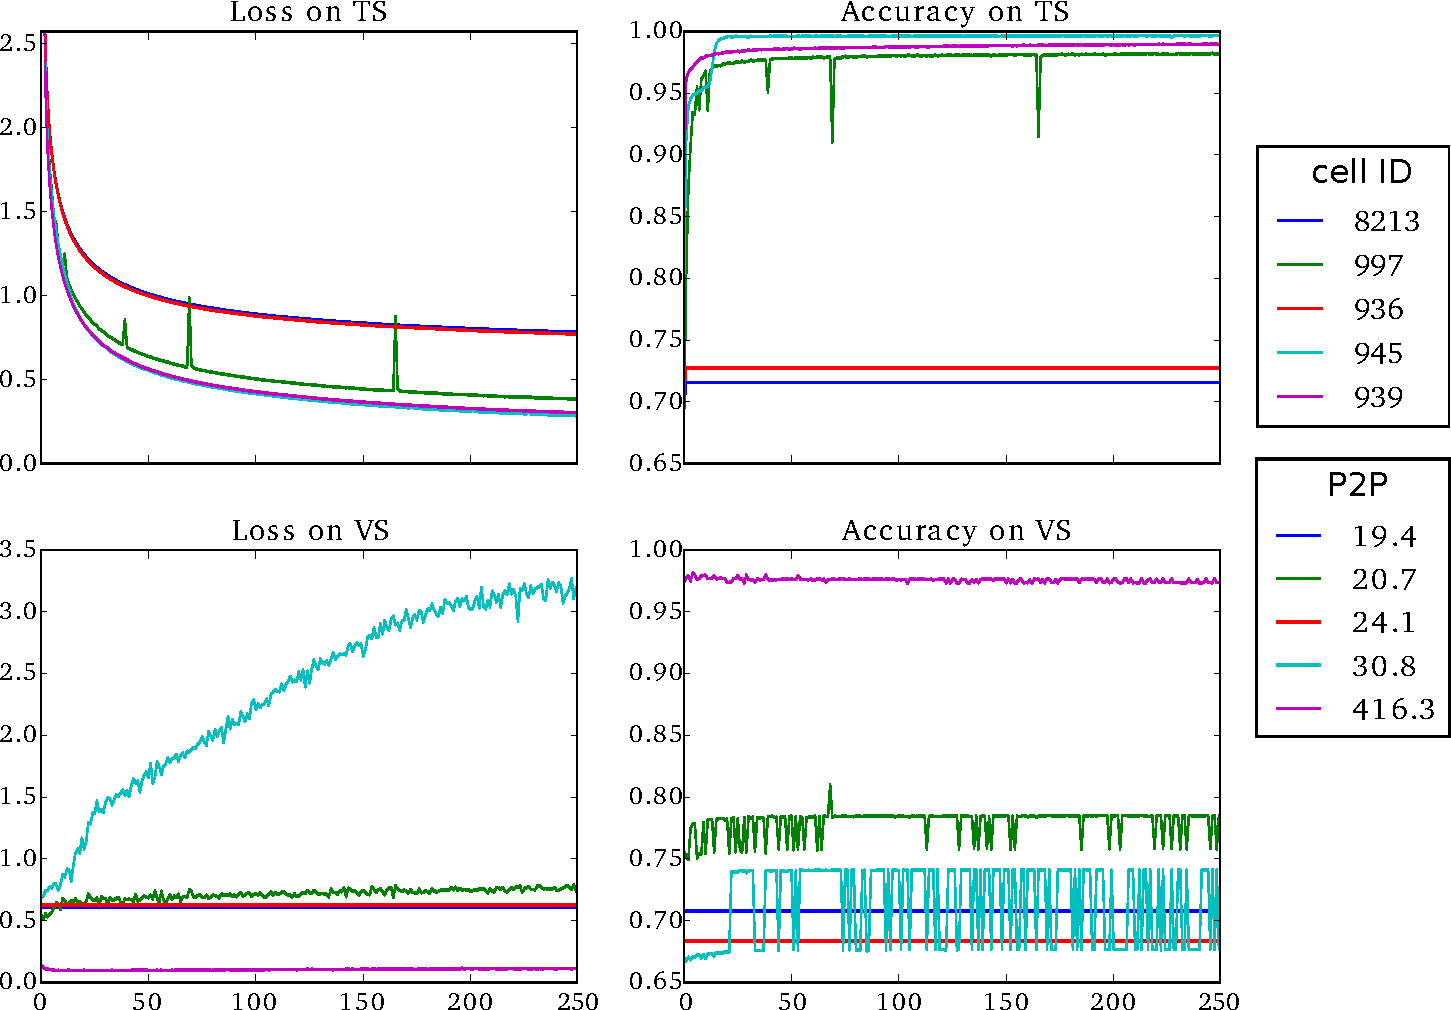
\includegraphics[width=\linewidth]{3.Chapter/study-on-different-cells-norm.pdf}
	\caption{Study on Different Recordings. Loss function and accuracies in the training set and in the validation set.The learning rate was $\eta = 0.01$, the weight decay was fixed at $\lambda = 0.001$, and the initialization method was LeCun Uniform. On the legend on the top is the Cell ID and on the legend on the bottom are the P2P amplitude (in $\mu V$).
}
\label{fig:study-cells}
\end{figure}

The values for the True Positives (TP), True Negatives (TN), False Positives (FP) and False Negatives (FN) at the end of traning were calculated as well as the values for the True Positive Rate (TPR), calculated as :
\begin{equation}
\centering
TPR = \frac{TP}{TP + FN}
\end{equation}

The results are presented in Table \ref{table:confusion-matrix}.

\begin{table}[htb]
\begin{center}
\begin{tabular}{c|cccc|cc}
cell ID & TP & TN & FP & FN & TPR & phy acc.\\ \hline
8213 & 0.00\% & 70.76\% & 0.00\% & 29.24\% & 0.00\% & -0.01\% \\
936 & 0.00\% & 68.35\% & 0.00\% & 31.65\% & 0.00\% & -1.02\% \\ 
939 & 26.85\% & 70.53\% & 0.38\% & 2.24\% & 92.31\% & 46.60\% \\ 
945 & 6.45\% & 67.66\% & 0.07\% & 25.81\% & 20.00\% & 8.38\% \\ 
997 & 2.67\% & 75.80\% & 0.18\% & 21.35\% & 11.11\% & 1.99\% \\ 
\end{tabular}
\end{center}
\caption{Values of the True Positives (TP), True Negatives (TN), False Positives (FP) and False Negatives (FN) at the end of the training, along with the value of the True Positive Rate (TPR). The accuracies achieved with phy in Chapter 2 are also presented. }
\label{table:confusion-matrix}
\end{table}

With the recordings 8213 and 936, the DNN converged to the "zero" solution since the very first epoch and was never able to be "trained out" of the local minimum it got held in. Indeed, in Table \ref{table:confusion-matrix}, the number of false negatives equals the fraction of "1" examples after upsampling (see Table \ref{table:summary-afterUS}).

The recordings 945 and 997 kept oscillating between two "states". In both cases the state with the lowest accuracy corresponds to the "zero" solution, successfully classifying all the "0" labeled examples but failing in the examples labeled as "1". In the other state, the network seems to positively classify 20.0\% and 11.11\% of the "1" examples, respectively.

Trained with the recording from the cell 939, the DNN managed to correctly classify 92.31\% of the EAPs present. 

\section{Discussion}
\label{sec:chap3-discussion}


Looking at Fig. \ref{fig:study-cells} it can be seen that with the chosen training configuration all recordings trained the DNN after only a few epochs: by the epoch 20 the accuracies in all cases reached their final value, or even getting worse afterwards, and therefore applying a stop criteria should be considered.

%%%%%%%%%%%%%%%%%%%%%%   COMPARISON WITH PHY    %%%%%%%%%%%%
Comparing with the results using phy presented in Chapter 2, this method seems to give better results: when the network didn't converge to the "zero" solution, the detection rates more than doubled, reaching a 5-fold increase on the recording 997. However, the detection rates on the recordings 945 and 997 correspond to the detection of only one spike, since the validation set in these case only had 5 and 9 different positive examples. 

It is also important to refer that the oscillations observed with the recording 945 and 997 suggest that the training used work may not be very robust: it appears that the network "jumps" easily between two local minima. Therefore it seems imperative to trained the network with more data. Another possible improvement would be increasing the probability parameter on the dropout procedure.

The recording 939 trained the network into detecting 92.31\%, which is a large value, with very few false positives and false negatives. However, in this recording the P2P amplitude was 416.3 $\mu V$, with a noise standard deviation of 10.51 $\mu V$, and should be easily detected with the conservative application of classic methods such as a threshold-based detection.
%Nonetheless, this method seems to be able to deal with situation of overlapping spikes. 
%As it was discussed in Chapter 2, probably the number of events detected by phy in this recording is underestimated and thus the improvement in this dataset may not be a big as it may seem.

In reality, the configurations and hyperparameters considered optimal were only studied with the recording 939 and may not be optimal for all datasets.

It should be noted that it is very likely that the windows labeled as "0" have many other spikes. This may actually make the training process much more difficult: since the production of any EAP relies on similar physical process, many spikes may be very similar to the spike from the juxta neuron, making the distinction, and thus the training, more difficult. For this reason, using a bigger dataset should return significantly better results, in particular, a bigger dataset with more different positive examples. The upsampling step may have forced the training to give a larger importance to each positive example but it didn't feed the network any new information about the event of interest. Possibly it could have been better to, instead of upsampling, perform downsampling or both: reduce the number of negative examples and increase the number of positive examples. In this way, more variability on the positive examples would be taken into consideration, making the network learn the useful structure of the EAPs better.

In the recording 8213 there were 202 different positive examples in the training set, more or less the same as in recording 939 which had 207. Nonetheless, the DNN was trained into the "zero" solution. At the same time this recording was the lowest in amplitude, with a $19.4 \mu V$ P2P amplitude, and the one with the highest noise standard deviation of $12.95 \mu V$, therefore most of the example are probably "drowned" in the noise, preventing the DNN to see the signal of interest. This suggests that there may be a threshold SNR below which this method cannot be applied, perhaps regardless of how many spikes there are in the training set.

It is important to keep in mind the question we're training the network to answer: whether or not, in a certain time window, there was a spike from this particular cell, and not a spike from any cell. Indeed, each network was trained with only one dataset individually. It would be interesting to train a DNN with different datasets recorded with the same probe. In this situation the question would be different: in this time window is a there a spike from this set of targeted cells? This would not only increase the number of examples (in particular positive examples), but also make this procedure more generalizable and applicable in more situations when enough different datasets have been used. However, this would affect the training: it may make it easier if the datasets are similar, or it may make it harder if there is a big difference in  EAPs from the considered juxta neurons. 
It is never too much noting that this new dataset would have to shuffled if the training algorithm doesn't do it for us, for instance if we train the network in chunks of data due to memory contraints. Otherwise, on the first epochs of training the DNN would "crystalize" on detecting that particular first EAP and may be harder to train it away from that configuration to learn the new EAPs. 
Another way to achieve this would be producing a hybrid dataset where many ground truth datasets are brought together, for examples as an average or hand-crafted, to produce one simulated recording with larger variability on the positive examples without increasing the size of the dataset, and therefore improving the unbalance in the dataset.

As mentioned above, due to memory constraints, the time windows were time shifted from the previous by 5 samples. Windows whose central sample were closest to each time juxta time where labeled as positives. Therefore if sequential time windows were presented, the DNN would probably yield 5  positive predictions per juxta spike.